\documentclass[crop,tikz]{standalone}
\usetikzlibrary{backgrounds}
\colorlet{blue}{cyan}
\tikzset{
  inverted/.style = {
    color=white,
    background rectangle/.style={fill},
    show background rectangle
  }
}

\usepackage{amsmath}
\tikzset{>=latex}
\usetikzlibrary{patterns,decorations.pathmorphing}

\begin{document}
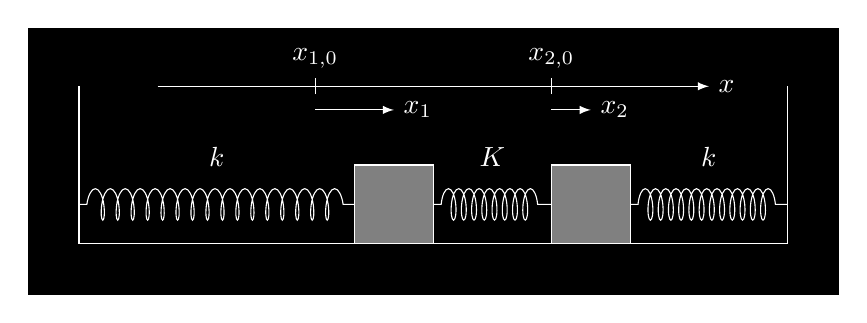
\begin{tikzpicture}[inverted,inverted]
  \pgfmathsetmacro{\thickness}{0.5};
  \pgfmathsetmacro{\hoehe}{2};
  \pgfmathsetmacro{\breite}{9};
  \pgfmathsetmacro{\xonenull}{3};
  \pgfmathsetmacro{\xtwonull}{6};
  \pgfmathsetmacro{\xone}{4};
  \pgfmathsetmacro{\xtwo}{6.5};
  \pgfmathsetmacro{\ynull}{2};
  \fill[pattern=north west lines] (0,\hoehe) -- (0,0) -- (\breite,0) -- (\breite,\hoehe) -- ({\breite+\thickness},\hoehe) -- ({\breite+\thickness},{-\thickness}) -- ({-\thickness},{-\thickness}) -- ({-\thickness},\hoehe) -- cycle;
  \draw (0,\hoehe) -- (0,0) -- (\breite,0) -- (\breite,\hoehe);
  \draw[fill=gray] ({\xone-0.5},0) rectangle ++ (1,1);
  \draw[fill=gray] ({\xtwo-0.5},0) rectangle ++ (1,1);
  \draw[decoration={aspect=0.3,segment length=1.9mm,amplitude=2mm,coil,pre length=1mm,post length=1mm},decorate] (0,0.5) -- ({\xone-0.5},0.5) node[above,pos=0.5,yshift=1em] {$k$};
  \draw[decoration={aspect=0.3,segment length=1.3mm,amplitude=2mm,coil,pre length=1mm,post length=1mm},decorate] ({\xone+0.5},0.5) -- ({\xtwo-0.5},0.5) node[above,pos=0.5,yshift=1em] {$K$};
  \draw[decoration={aspect=0.3,segment length=1.3mm,amplitude=2mm,coil,pre length=1mm,post length=1mm},decorate] ({\xtwo+0.5},0.5) -- (\breite,0.5) node[above,pos=0.5,yshift=1em] {$k$};
  \draw[->] (1,\ynull) -- ({\breite-1},\ynull) node[right] {$x$};
  \draw (\xonenull,{\ynull-0.1}) -- ++ (0,0.2) node[above] {$x_{1,0}$};
  \draw ({\xtwonull},{\ynull-0.1}) -- ++ (0,0.2) node[above] {$x_{2,0}$};
  \draw[->] (\xonenull,{\ynull-0.3}) -- ++ ({\xone-\xonenull},0) node[right] {$x_1$};
  \draw[->] (\xtwonull,{\ynull-0.3}) -- ++ ({\xtwo-\xtwonull},0) node[right] {$x_2$};
\end{tikzpicture}
\end{document}
